\documentclass[aspectratio=43]{beamer}
\usepackage[utf8]{inputenc}

%%%%%%%%%%%%%%%%%%%%%%%% THEME
\usetheme{material}
\useLightTheme
\usePrimaryTeal
\useAccentGreen

\usepackage{macros} % must come after theme

\title{Hello \qw}
\keywords{\qm,\qc}

\begin{document}

\begin{frame}
	\titlepage
\end{frame}


\begin{frame}{Table of contents}
	\begin{card}
		\tableofcontents
	\end{card}
\end{frame}

\section{Motivation}
\begin{frame}{Motivation}
\begin{card}[Why]
    \begin{chapquote}[2pt]{\href{https://en.wikipedia.org/wiki/Seth_Lloyd}{Seth Lloyd}}
        ``Classical computation is like a solo voice - one line of pure tones succeeding each other. Quantum computation is like a symphony - many lines of tones interfering with one another.''
    \end{chapquote}
\end{card}

\pagenumber
\end{frame}

\begin{frame}{Motivation}
\begin{card}[How]
    \qc can be seen as leveraging the phenomena that happen at the atomic and subatomic levels - in the \qw\xspace- to produce computations that, ultimately, surpass \cc.
\end{card}
\pagenumber
\end{frame}

\begin{frame}{About this course}
\begin{card}
    This course is suited for beginners in \qm and \qc. If you are already familiar with the concepts of a given week, you are encouraged to move forward in the course. 
    
    This course brings novelty in that it focuses on \textbf{learning by doing}, and that is why you will also learn about \qk and \ibmqe.
    
    The author believes both that learning should be fun and that derision is a wonderful attention gripper, so humour will be used as the powerful tool that it is, wisely.
\end{card}
\pagenumber
\end{frame}

\begin{frame}{About this course - Study plan}
\begin{card}
    \begin{itemize}
        \item \qm 101
        \item \qk and \ibmqe
        \item \qi
        \item Designing \qcts
        \item \qa (Deutsch, Grover, Shor)
        \item \qc applications
        \item \q Computers - state of the art
        \item Implications and ethical considerations throughout
    \end{itemize}
\end{card}
\pagenumber
\end{frame}

\section{Introduction}
\begin{frame}{Introduction}
\begin{card}
    In this first week, we will start by defining what \qc is and how it compares to \cc. Next, a walk-through the novelty that \qm brings and how it compares to \cp.  As a starting point to understanding how these quantum properties can be used to tackle problems algorithmically, we will introduce the concepts of \textbf{superposition} and \textbf{measurement}, that of \textbf{entanglement} will be introduced later, at a stage where it makes more sense and is easier to assimilate.
\end{card}
\pagenumber
\end{frame}


\section{\qp vs \cp}

\begin{frame}{\cp}
\begin{card}
    \cp (also \cm) describes the world \textit{as we see it}, in its macro level. Some of its properties:
    \begin{description}
        \item[size] objects with $size \gtrsim 1nm\ (10^{-9}m)$
        \item[speed] objects of $speed \lesssim \speedoflight$
    \end{description}
\end{card}
\pagenumber
\end{frame}


\begin{frame}{\qp}
\begin{card}
    \qp (also \qm) describes the world \textit{as we see it}, in its macro level. Some of its properties:
    \begin{description}
        \item[size] objects with $size \lesssim 1nm$
        \item[speed] objects of $speed \lesssim \speedoflight$
    \end{description}
\end{card}
\pagenumber
\end{frame}

\begin{frame}{The kingdoms of \cl and \qm}
\begin{card}
    \centering\cardImg{classical_vs_quantum_dimensions.png}{\textwidth}
\end{card}
\pagenumber
\end{frame}

\section{Principles of \qm}
\subsubsection{\qsp}
\begin{frame}{\qsp}
    \begin{card}
        A \q state (of a particle) can be seen as being composed by more than one different states, simultaneously. It is not in state A \textbf{or} B, it is in state A \textbf{and} state B, at the same time. This defies classical views of the world, where two things are never true at the same time and requires some mental effort!\\
        The state is, therefore, in a kind of superposition.
    \end{card}
\pagenumber
\end{frame}

\begin{frame}{\qsp - Schrödinger's cat}
    \textbf{Thought experiment:} Imagine a cat locked inside a box, along with a poison releasing mechanism. The mechanism has a 50\% chance of having been activated at the time the box is about to be opened. At that moment, we cannot be sure of the cat's living state. Perhaps, we should assume the cat is both dead and alive, at the same time. With each state having the same probability.
    \begin{center}
	    \cardImg{img/cat.png}{0.5\textwidth}
    \end{center}
    \begin{center}
        To worlds, inside one.
    \end{center}
\pagenumber
\end{frame}


\begin{frame}{\qsp}
    \begin{cardTiny}
        Formally, such states are represented using the \textbf{Ket notation} (as defined by \textit{Paul Dirac}). State 0 would be \ket{0}. 
    \end{cardTiny}
    \begin{cardTiny}
        \begin{multicols}{2}
    		Consider the electron of a Hydrogen atom, orbiting around the nucleus, with only two (simplification) possible energy states. As this is a \q particle, these energy states are quantized, that is, they take only discrete (quantified) values. 
    		\begin{center}
    		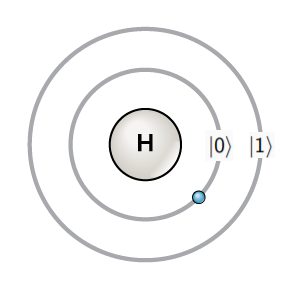
\includegraphics[width=0.4\textwidth]{hydrogen}
    		\end{center}
	    \end{multicols}
    \end{cardTiny}
\pagenumber
\end{frame}

\begin{frame}{\qsp}
    \begin{card}
        When we have no evidence of the electron's state, we assume that it is in a superposition of both positions. This \qsp $\ket{\phi}$ is written as:
	\begin{equation*}
	    \superpos
	\end{equation*}
    \end{card}
    \begin{cardTiny}
        $\alpha$ and $\beta$ represent how likely each of the two states is. These are complex numbers such that $|\alpha|^2 + |\beta|^2 = 1$. 
    \end{cardTiny}
    \begin{cardTiny}
        \small{
        So, why and how does \qsp actually work?\\ \textbf{We do not know!} (this statement pops up frequently in \q) However, some \href{https://arxiv.org/abs/1707.09483}{interesting experiments} might just be able to answer us soon enough...
        }
    \end{cardTiny}
\pagenumber
\end{frame}

\begin{frame}{\qsp\space-  Plane representation}
    \begin{cardTiny}
        \begin{multicols}{2}
    		Another important remark to make is that a superposition can be projected as unit vector onto a 2D plane (even though $\alpha$ and $\beta$ are complex numbers). In essence, this allows us to convert a superposition in the $\ket{0}\ket{1}$ basis, as is $\ket{\psi}$, onto other basis. Basis are orthonormal.
    		\begin{center}
                

\tikzset{every picture/.style={line width=0.75pt}} %set default line width to 0.75pt        

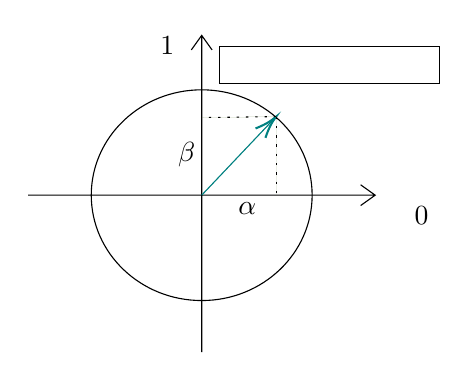
\begin{tikzpicture}[x=0.75pt,y=0.75pt,yscale=-1,xscale=1]
%uncomment if require: \path (0,240.1999969482422); %set diagram left start at 0, and has height of 240.1999969482422

%Shape: Axis 2D [id:dp5007372493556268] 
\draw  (187.65,86.57) -- (354.8,86.57)(271.23,9.59) -- (271.23,162.2) (347.8,81.57) -- (354.8,86.57) -- (347.8,91.57) (266.23,16.59) -- (271.23,9.59) -- (276.23,16.59)  ;
%Shape: Ellipse [id:dp25953493006417205] 
\draw   (218.02,86.57) .. controls (218.02,58.53) and (241.84,35.81) .. (271.23,35.81) .. controls (300.61,35.81) and (324.43,58.53) .. (324.43,86.57) .. controls (324.43,114.61) and (300.61,137.34) .. (271.23,137.34) .. controls (241.84,137.34) and (218.02,114.61) .. (218.02,86.57) -- cycle ;
%Straight Lines [id:da7303300795271543] 
\draw [color={rgb, 255:red, 0; green, 128; blue, 128 }  ,draw opacity=1 ][fill={rgb, 255:red, 0; green, 120; blue, 120 }  ,fill opacity=1 ]   (271.23,86.57) -- (305.71,50.19) ;
\draw [shift={(307.08,48.74)}, rotate = 493.47] [color={rgb, 255:red, 0; green, 128; blue, 128 }  ,draw opacity=1 ][line width=0.75]    (10.93,-3.29) .. controls (6.95,-1.4) and (3.31,-0.3) .. (0,0) .. controls (3.31,0.3) and (6.95,1.4) .. (10.93,3.29)   ;

%Straight Lines [id:da4416217930551922] 
\draw [fill={rgb, 255:red, 77; green, 108; blue, 42 }  ,fill opacity=1 ] [dash pattern={on 0.84pt off 2.51pt}]  (307.08,48.74) -- (307.08,86.21) ;


%Straight Lines [id:da8036276031325384] 
\draw [fill={rgb, 255:red, 77; green, 108; blue, 42 }  ,fill opacity=1 ] [dash pattern={on 0.84pt off 2.51pt}]  (307.08,48.74) -- (271.12,49.16) ;



% Text Node
\draw (377.16,96.17) node  [align=left] {$\ket{0}$};
% Text Node
\draw (254.65,14.61) node  [align=left]{$\ket{1}$};
% Text Node
\draw (293.22,93.23) node  [align=left] {$\alpha$};
% Text Node
\draw (263.96,66.78) node  [align=left] {$\beta$};

% Text Node
\draw    (279.6,14.8) -- (385.6,14.8) -- (385.6,32.8) -- (279.6,32.8) -- cycle  ;
\draw (332.6,23.8) node [scale=0.8] [align=left] {$\superpos$};

\end{tikzpicture}

    		\end{center}
	    \end{multicols}
    \end{cardTiny}
\pagenumber
\end{frame}

\begin{frame}{\qsp\space- Vector representation}
    \begin{cardTiny}
        Moreover, a quantum state $\superpos$ can be seen as a unit vector in the complex bi-dimensional space ($\mathbb{C}^2$) \begin{bmatrix}$\alpha$ \\ $\beta$\end{bmatrix}, such that:
        \begin{equation*}
            \alpha \ket{0} + \beta \ket{1} = 
            \begin{bmatrix}$\alpha$ \\ $\beta$\end{bmatrix}^\intercal 
            \times
            \begin{bmatrix}1 & 0\\ 0 & 1\end{bmatrix}
        \end{equation*}
        Given the following as the basis vectors (this is the zero-one basis):
        \begin{equation*}
            \ket{0} =  \begin{bmatrix}1 \\ 0\end{bmatrix},\\
            \ket{1} =  \begin{bmatrix}0 \\ 1\end{bmatrix}
        \end{equation*}
    \end{cardTiny}
\pagenumber
\end{frame}

\begin{frame}{\qsp\space- Basis}
    \begin{multicols}{2}
        As a matter of fact, any linearly independent pair of unit vectors can act as basis. One well known basis is the $\ket{+}\ket{-}$ (plus-minus) basis:
        \begin{equation*}
            \ket{+} =  \begin{bmatrix}\osqrt \\ \osqrt\end{bmatrix},\\
            \ket{-} =  \begin{bmatrix}\osqrt \\ -\osqrt\end{bmatrix}
        \end{equation*}
        This is simply the $\ket{0}\ket{1}$ basis rotated by $\frac{\pi}{4}$($45º$).
		\begin{center}
            

\tikzset{every picture/.style={line width=0.75pt}} %set default line width to 0.75pt        

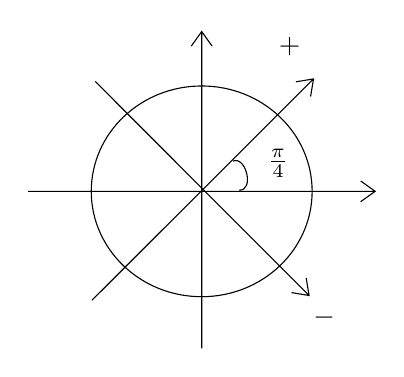
\begin{tikzpicture}[x=0.75pt,y=0.75pt,yscale=-1,xscale=1]
%uncomment if require: \path (0,240.1999969482422); %set diagram left start at 0, and has height of 240.1999969482422

%Shape: Axis 2D [id:dp5007372493556268]
\draw  (187.65,86.57) -- (354.8,86.57)(271.23,9.59) -- (271.23,162.2) (347.8,81.57) -- (354.8,86.57) -- (347.8,91.57) (266.23,16.59) -- (271.23,9.59) -- (276.23,16.59)  ;

%Shape: Ellipse [id:dp25953493006417205] 
\draw   (218.02,86.57) .. controls (218.02,58.53) and (241.84,35.81) .. (271.23,35.81) .. controls (300.61,35.81) and (324.43,58.53) .. (324.43,86.57) .. controls (324.43,114.61) and (300.61,137.34) .. (271.23,137.34) .. controls (241.84,137.34) and (218.02,114.61) .. (218.02,86.57) -- cycle ;
%Shape: Axis 2D [id:dp6909779044773345] 
\draw  (219.93,33.62) -- (322.97,136.77)(325.11,32.4) -- (218.33,139.07) (321.56,128.28) -- (322.97,136.77) -- (314.49,135.35) (316.62,33.81) -- (325.11,32.4) -- (323.69,40.89)  ;
%Curve Lines [id:da10382465930858809] 
\draw    (286.27,72) .. controls (292.68,69.4) and (296.68,86.4) .. (289.27,86) ;



% Text Node
\draw (330.16,147.17) node  [align=left] {$\ket{-}$};
% Text Node
\draw (313.65,16.61) node  [align=left] {$\ket{+}$};
% Text Node
\draw (308,73) node  [align=left] {$\frac{\pi}{4}$};


\end{tikzpicture}

		\end{center}
    \end{multicols}
\pagenumber
\end{frame}




\subsubsection{\qmt}
\begin{frame}{\qmt}
    \begin{cardTiny}
        From a pragmatic perspective, what happens when we open the box and look at the cat? From that moment on, only one state remains, either death \textbf{or} life. And we cannot close the box again and expect a different outcome.
    \end{cardTiny}
    \begin{cardTiny}
        \centering\textit{The cat is out of the box.}
    \end{cardTiny}
    \begin{cardTiny}
        A \textbf{Measurement} causes the system to stabilise, in a non-reversible way. When we perform a measurement  on the electron's state (let this process be a technicality, for now), we get $\ket{0}$ \textbf{or} $\ket{1}$. If we repeat the measurement, the result will be the same, \textbf{always}. 
    \end{cardTiny}
\pagenumber
\end{frame}

\begin{frame}{\qmt}
\begin{cardTiny}
\small{
    To better understand what a measurement is, it is important to understand that it is \textbf{basis-specific}, meaning we could measure on the $\ket{0}\ket{1}$ or on the $\ket{+}\ket{-}$ basis (or another \href{http://mathworld.wolfram.com/LinearlyIndependent.html}{LI}). Example:\\
    You have a qubit in a superposition $\osqrt\alpha+\osqrt\beta$, you measure (zero-one basis) it into a bit and the result is 0 (horizontal). Now, if you convert it to the plus-minus basis you will get $\psi = \osqrt\ket{+} + \osqrt\ket{-}$.\\
    Imagine that the measurement had not happened and was instead performed on the plus-minus basis, the result would be $+$ (since $\ket{+}=\osqrt\ket{0}+\osqrt\ket{1}$).
}
\end{cardTiny}
\begin{cardTiny}
    \small{You can now see the impact of choosing a given basis to perform a measurement. We will return to this later, the simple notion of this consideration is what you should absorb now.}
\end{cardTiny}
\pagenumber
\end{frame}

\begin{frame}{\qmt}
\begin{cardTiny}
\small{
    Pragmatically speaking, \qmt requires a few considerations. Firstly, it produces a single output form a state that is stochastic, meaning that doing it once is not enough to be sure of the probability distribution. So, typically, each experiment is executed a large number of times (hundreds and sometimes thousands) so that the confidence in the results meets the expectations.\\
    Furthermore, as you will see when deploying to real quantum devices, current experimental setups are not perfect (and hardly ever will be) so even the simplest of programs may produce buggy results and a \q Scientist should be aware of it.\\As a matter of fact \href{https://quantumexperience.ng.bluemix.net/qx/editor}{\ibmqe}'s devices are usually well described even in the average error (noise) ratios you should expect.
}
\end{cardTiny}
\pagenumber
\end{frame}

\section{Why \q?}
\begin{frame}{Why \q?}
    To end this introductory week to the \qw, there are a few useful considerations to make:
    \begin{itemize}
        \item \qc is worth our time because it brings the promise of revolutionising the amount of computation within human reach, from tackling currently impossible problems to rendering most encryption standards useless.
        \item \qc works because it allows for the massive parallelisation of computations hitherto unattainable with such ease in \cc, because humans are not defining this parallelism, Mother Nature is! That and the \qm at play (some yet to see) give it even more out-of-the-box characteristics adding to its enormous potential. 
    \end{itemize}
\pagenumber
\end{frame}

\begin{frameImg}[width]{dilbert}


\end{frameImg}

\section{Where to learn more?}
\begin{frame}{Where to learn more?}
\begin{card}
    \begin{itemize}
        \item \href{https://www.quantiki.org/wiki/introduction-quantum-theory}{Introduction to Quantum Theory, Quantiki}
        \item \href{https://www.khanacademy.org/science/physics/quantum-physics/quantum-numbers-and-orbitals/a/the-quantum-mechanical-model-of-the-atom}{Khan Academy, The quantum mechanical model of the atom}
        \item \href{https://www.goodreads.com/book/show/331680.Programming_the_Universe}{Programming the Universe: A Quantum Computer Scientist Takes on the Cosmos}
        \item \href{https://www.goodreads.com/book/show/260142.The_Principles_of_Quantum_Mechanics}{The Principles of Quantum Mechanics, \textit{Paul Dirac}}
    \end{itemize}
\end{card}
\end{frame}

\end{document}
